
\chapter{Делаем Компоненты красивыми}

Наш путь по лучшим практикам и паттернам React пришел к моменту, когда мы хотим сделать наши компоненты красивее. Для этого мы разберемся с вопросом, почему обычный CSS не всегда является наилучшим вариантом для стилизации компонент, и какие есть альтернативы.

Мы начнем со встроенных стилей, библиотеки Radium, CSS модулей и Styled Compopnents, а затем детально разберем волшебство CSS в JavaScript.

Вопрос стилизации в React стоит очень горячо и вызывает множество споров, поэтому эта глава требует непредвзятости и готовности оценить плюсы и минусы различных инструментов.

В этой главе мы рассмотрим следующие вопросы:

\begin{itemize}
	\item Общие проблемы масштабируемости CSS
	\item Встроенные стили в React и их отрицательные стороны
	\item Как библиотека Radium помогает исправить проблемы встроенных стилей
	\item Как настроить проект с нуля для работы с Webpack и CSS Модулей
	\item Возможности CSS Модулей и их преимущества перед глобальными стилями
	\item Современный подход к стилизации компонентов с библиотекой Styled Components
\end{itemize}

\section{CSS in JS}

Многие знают, что для стилизации в React переломный момент произошел в Ноябре 2014 года, когда \textit{Кристофер Шедо (Christopher Chedeau)} выступил на конференции NationJS.

Кристофер, также известный в интернете как \textit{Vjeux}, работает в Facebook и способствует развитию React. На этой конференции он рассказал о проблемах с CSS при масштабировании приложений, которые они встретили в Facebook.

Важно знать об этих проблемах, так как многие из них часто встречаются на практике, а также будет легче понять необходимость разных концепций, таких как \textbf{встроенные стили} и \textbf{локальные классы}.

На слайде вы можете увидеть один из слайдов с этой презентации со списком главных проблем с CSS:

\begin{figure}[hbt]
  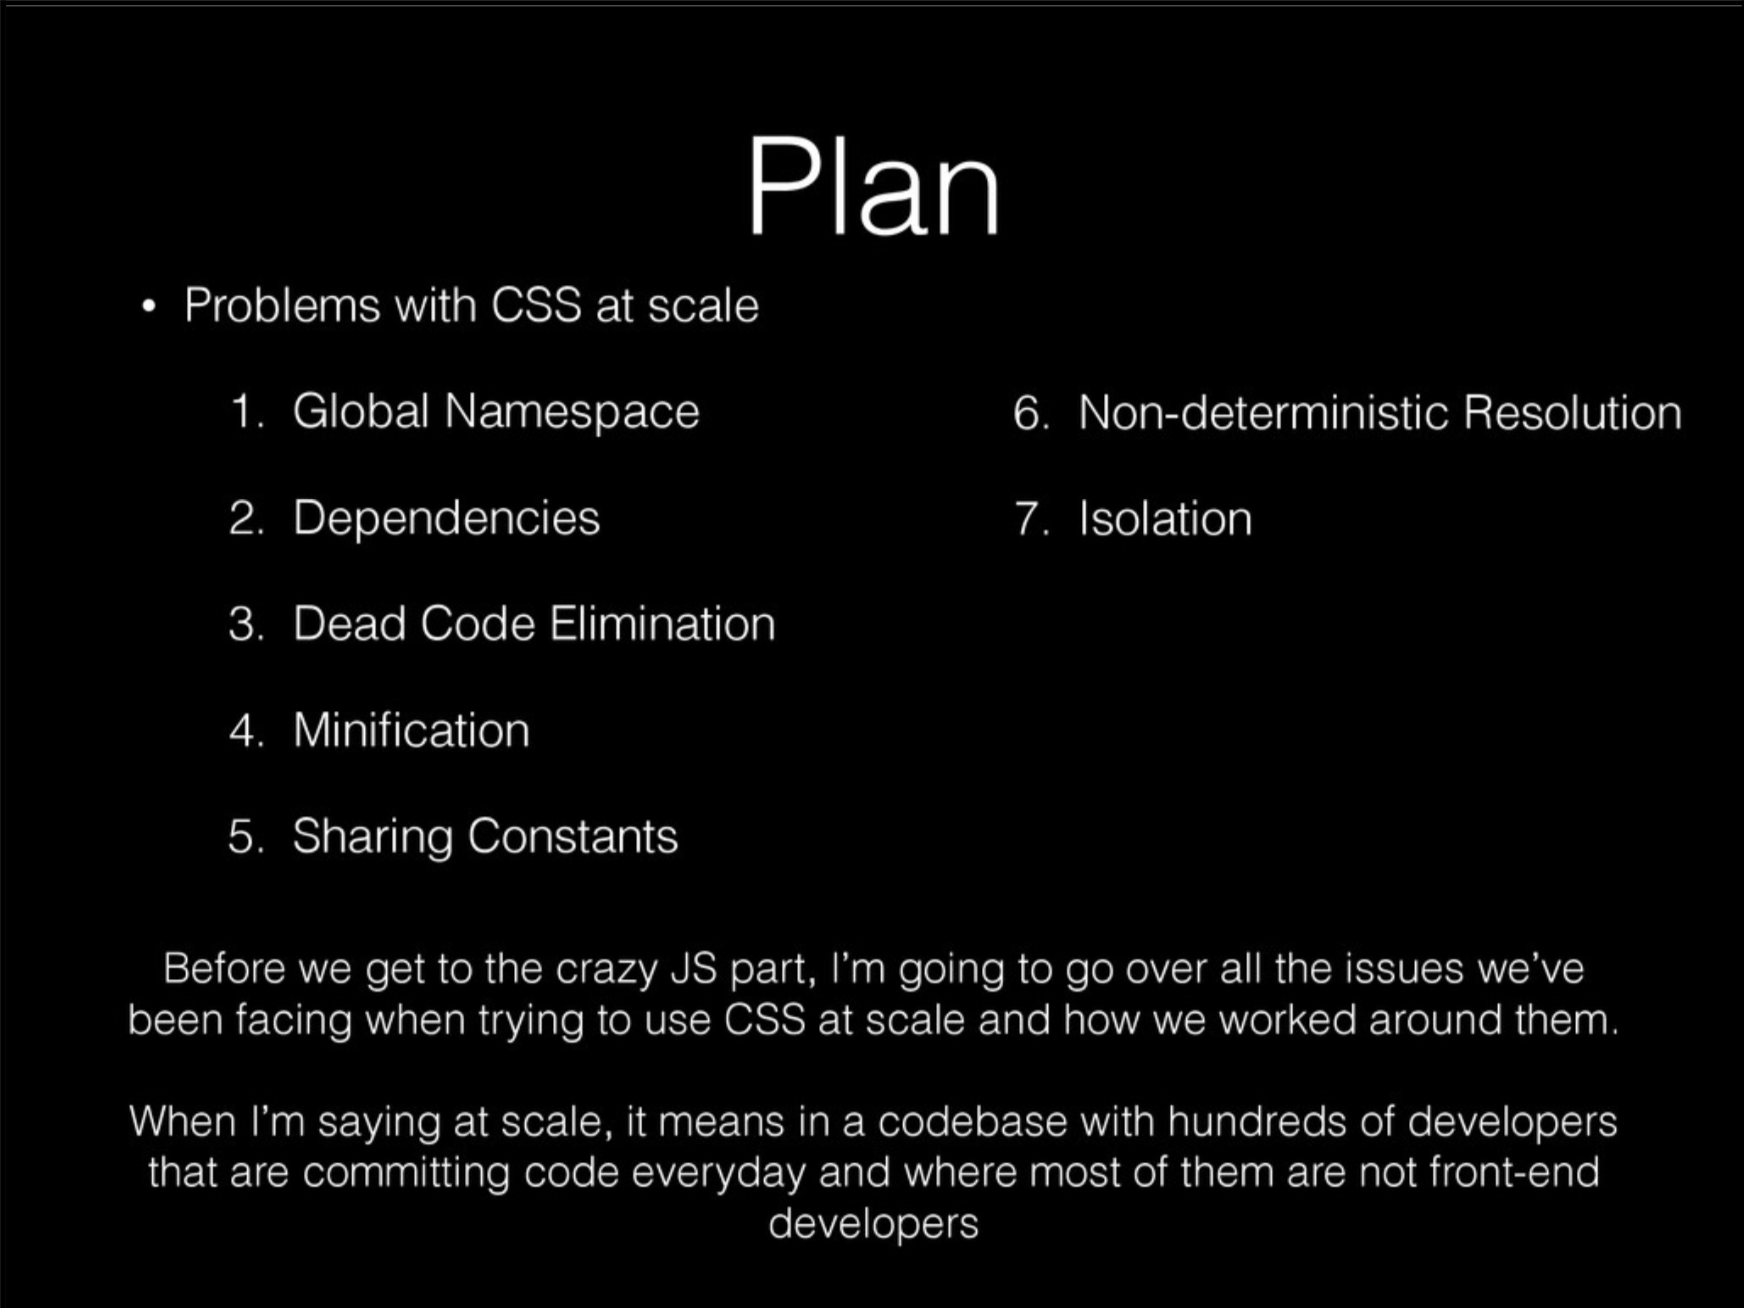
\includegraphics[width=1.\textwidth]{images/css-problems-slide}
\end{figure}

Первая и хорошо известная проблема CSS заключается в глобальных селекторах. Не важно, как вы организовали свой код, использовали ли пространства имен или BEM методологию, в конце все равно стили окажутся в одном глобальном пространстве имен. И это ошибка не только идеологически, это ведет к множеству ошибок и ухудшает поддерживаемость большой кодовой базы. Когда мы работаем в больших командах, не так просто знать о существовании конкретного класса или стилизованного элемента, что ведет к добавлению большего количества классов вместо переиспользования существующих.

Следующая проблема относится к определению зависимостей. На деле бывает очень сложно понять, от каких именно стилей зависит конкретный компонент. Так как стили глобальны, они могут использоваться из любых компонентов, а любой компонент может использовать любые стили. В таких условиях может быть очень легко потерять контроль.

Фронтенд разработчики привыкли использовать препроцессоры для разделения CSS на модули, но в итоге для браузера все равно генерируется большой CSS бандл. Так как объем кода CSS быстро растет, мы получаем еще одну проблему с \textbf{удалением неиспользуемого кода (dead code elimination)}. Так как сложно понять, какой стиль к какому компоненту относится, задача удаления неиспользуемого кода становится еще сложнее. Также, если учесть каскадную природу CSS, удаление любого селектора или правила может привести к непредсказуемым последствиям в браузере.

Минификация селекторов и имен классов также добавляет головной боли и в CSS и в JavaScript приложение. Хотя на первый взгляд эта задача кажется простой, на деле все усложняется, когда классы добавляются во время исполнения программы или высчитываются на клиенте.

Отсутствие возможности минифицировать CSS сильно сказывается на производительности, так как может значительно сказаться на размере CSS файлов.

Также в рамках обычного CSS нетривиально создать константы, общие для CSS и JavaScript. Например для случаев, когда мы хотим знать высоту заголовка, чтобы рассчитать расположение элементов относительно него.

Обычно, JavaScript API используется для получения нужных значений, однако было бы значительно оптимальней использовать общие константы и избежать дорогих вычислений во время исполнения программы. Это и есть пятая проблема, которую Vjeux и другие разработчики Facebook попытались решить.

Шестая проблема заключается в недетерминированный обработке файлов CSS. По факту, в CSS важен порядок обработки файлов с исходным кодом. Таким образом, если файлы грузятся по требованию, то сохранение их порядка не гарантируется, что ведет к применению неверных стилей к компонентам. 

Предположим, что мы хотим оптимизировать загрузку CSS и загружать стили для конкретной страницу только тогда, когда пользователь открывает эту страницу. Если стили для последней страницы содержат правила для  остальной части приложения, то отображение всего приложения может измениться. Например, если пользователь вернется по истории к предыдущей странице, она может несколько отличаться от того, что было до этого.

Очень сложно контролировать различные комбинации стилей, правил и путей, но возможность загружать CSS по мере необходимости критична для производительности приложения.

И седьмая проблема, о которой говорит Кристофер Шедо, связана с изоляцией компонент. В CSS очень сложно добиться изоляции файлов или компонентов между собой. Так как селекторы глобальны, они могут быть легко перезаписаны. Это нетривиальная задача, определить финальные стили компонента по примененным к нему классам, так как любой компонент может быть затронут любыми стилями, находящимися в приложении.

Я рекомендую посмотреть это выступление, если вы хотите узнать больше о проблемах масштабируемости CSS. Даже если этот вопрос выглядит сложным и противоречивыми, стоит открыто подходить к нему, чтобы найти решение, которое лучше всего подойдет в вашем случае:

\begin{quotation}
https://vimeo.com/116209150	
\end{quotation}

В заключение этого выступления было сказано, что для решения этих проблем масштабирования CSS в Facebook остановились на использовании \textit{встроенных стилей (inline styles)}.

В следующей части мы рассмотрим, как использовать встроенные стили в React, и какие есть плюсы и минусы у этого подхода.

\section{Встроенные стили}

Документация React советует разработчикам использовать встроенные стили для стилизации компонент. Это выглядит странно, так как за прошедшие годы мы усвоили, что разделение ответственности это хорошо, и мы не должны смешивать разметку и CSS.

React пытается изменить взгляд на разделение ответственности с привычного разделения технологий на разделение компонент. Разделение разметки, стилей и логики на разные файлы, которые сильно связаны и не могут работать по отдельности, иллюзия. Даже если это делает структуру чище, это не приносит реальной выгоды.

В React мы комбинируем компоненты, которые являются базовыми блоками для создания приложения. Мы можем переносить блоки по всему приложению и, независимо от того, где используются компоненты, они должны предоставлять одинаковую логику и отображение.

Это одна из причин, почему объединение стилей с компонентом с помощью встроенных стилей может иметь смысл в React.

Прежде всего посмотрим, как вообще использовать встроенные стили в React компонентах. Создадим кнопку с текстом \textbf{Click me!} и изменим у нее цвета фона и текста:

\begin{lstlisting}
const style = {
  color: 'palevioletred',
  backgroundColor: 'papayawhip',
}

const Button = () => <button style={style}>Click me!</button>
\end{lstlisting}

Как вы видите, использовать встроенные стили очень просто. Нам достаточно создать объект, в котором будут пары ключей и значений как в обычном CSS.

Единственный нюанс, правила с дефисом в названии должны быть записаны в горбатом регистре, а значения передаваться как строки, то есть в кавычках.

Есть несколько отличий при использовании вендорных префиксов. Например, если мы хотим определить переход (transition) в \textbf{webkit}, мы должны использовать атрибут WebkitTransition, который начинается с заглавной буквы. Это правило работает для всех вендорных префиксов кроме \textbf{ms}, которой должен быть в нижнем регистре.

Помимо этого, числа могут использовать без кавычек и единиц измерения, тогда они будут считаться пикселями.

Следующий фрагмент стилей устанавливает высоту в $100px$:

\begin{lstlisting}
const style = {
  height: 100,
}
\end{lstlisting}

Встроенные стили не только прекрасно работают, но и позволяют делать вещи, которые сложно сделать в CSS. Например, мы можем пересчитать значения стилей на клиенте во время исполнения, что мы увидим в следующим примере.

Предположим, что мы хотим создать поле ввода, размер шрифта в котором будет зависеть от его значения. То есть если значение поля будет равно 24, то и размер шрифта должен быть 24 пикселя. Сделать это с помощью CSS невозможно, также нужно приложить значительные усилия, чтобы сделать это в JavaScript.

Посмотрим, как легко сделать это со встроенными стилями.

Нам нужно будет хранить состояние компонента, поэтому создадим для него класс:

\begin{lstlisting}
class FontSize extends React.Component
\end{lstlisting}

В конструкторе класса определим начальное значение компонента, а также привяжем обработчик событий ввода к экземпляру этого класса:

\begin{lstlisting}
constructor(props) {
  super(props)
  
  this.state = {
    value: 16,
  }
  
  this.handleChange = this.handleChange.bind(this)
}
\end{lstlisting}

Мы создадим простой обработчик, который будет только обновлять состояние компонента в соответствии с вводимыми пользователем данными:

\begin{lstlisting}
handleChange({ target }) {
  this.setState({
    value: Number(target.value),
  })
}
\end{lstlisting}

И в конце мы создаем поле ввода с числовым типом, значение которого контролируется нашим компонентом через значение состояния и обработчик событий ввода.

Также мы передадим в атрибут $style$ этого поля ввода объект с актуальным значение размера шрифта. Как говорилось выше название правило должно быть в горбатом регистре, то есть мы должны определить параметр $fontSize$:

\begin{lstlisting}
render() {
  return (
    <input
      type="number"
      value={this.state.value}
      onChange={this.handleChange}
      style={{ fontSize: this.state.value }}
    />
  )
}
\end{lstlisting}

Как мы видим, при изменении значения поля ввода обновляется состояние компонента, что влечет за собой перерисовку компонента. В момент перерисовки значение размера шрифта берется из состояния компонента, которое берется из состояния. Таким образом размер шрифта меняется вслед за значением поля ввода. 

Как и у любого другого решения у встроенных стилей есть свои плюсы и минусы. И в данном случае последних не мало.

Например, со встроенными стилями невозможно использовать псевдоклассы (такие как $:hover$) и псевдоэлементы, что является большим ограничением, если вы хотите создать интерактивный и анимированный UI.

Есть множество костылей (workarounds), которые вы можете использовать для обхода этих ограничений. Например вы можете обычные элементы вместо псевоэлеменов, но для симуляции поведения CSS придется использовать CSS, что не оптимально.

То же самое относится и к \textbf{Медиа запросам (Media queries)}, которые нельзя определить с помощью встроенных стилей, что затрудняет создание адаптивного интерфейса. Также, так как стили передаются через JavaScript объект, во встроенных стилях невозможно использовать style fallbacks:

\begin{lstlisting}
display: -webkit-flex;
display: flex;
\end{lstlisting}

Все из-за того, что JavaScript объекты не могут содержать два атрибута с одинаковым именем. По этой причине использовать style fallbacks невозможно, хотя было бы хорошо иметь возможность их использовать при необходимости.

Еще одна возможность CSS, которую невозможно использовать через встроенные стили, это \textbf{Анимации}. Основной костыль (workaround) в этом случае, определить анимации глобально и использовать их внутри атрибута элементов $style$.

После использования встроенных стилей для предопределения стилей из CSS мы вынуждены использовать ключевое слово $!important$, что является плохой практикой, так как предотвращает применение других стилей к элементу.

И самое ужасное, что происходит при использовании встроенных стилей, это значительное усложнение отладки приложения. Мы вынуждены использовать названия классов для поиска элементов через DevTools браузера в целях отладки и проверки, какие стили были применены.

При использовании встроенных стилей все созданные стили окажутся в атрибуте $tyle$ созданного HTML элемента, что усложняет их отладку.

Например, кнопка из предыдущего примера будет отображена в следующий элемент:

\begin{lstlisting}
<button style="color: palevioletred; background-color: papayawhip;">Click me!</button>
\end{lstlisting}

Один такой элемент несложно прочитать, но представьте, что будут сотни таких элементов стилей. В этот момент это начинает превращаться в проблему.

Предположим, вы отлаживаете список таких элементов, в котором у каждого элемента своя копия стилей. При изменении одного элемента в браузере вы увидите, что меняется только редактируемый элемент, а все соседние элементы остаются неизменными. 

И помимо всего этого, если вы рендерите приложение на стороне сервера (подробнее мы поговорим об этом в Главе 8), то при использовании встроенных стилей размер страницы будет значительно больше. 

Алгоритмы сжатия могут достаточно сильно сжать получившийся HTML, так как в нем будет много повторяющихся частей, в некоторых случаях загрузка критичной части CSS может быть даже хорошей идеей, но в целом мы должны стремиться избежать этого.

Таким образом мы приходим к тому, что встроенные стили создают проблем больше чем решают.

По этим причинам сообщество создало другие инструменты для решения проблем встроенных стилей, не теряя при этом объединения стилей с компонентами. 

После выступления Кристофера Шедо множество разработчиков задумались о проблеме встроенных стилей и начали искать новые решения для использования CSS в JavaScript.

Автор книги изучил все из них и опубликовал репозиторий, в котором создал простую кнопку с помощью каждого из этих методов:

\begin{quotation}
https://github.com/MicheleBertoli/css-in-js
\end{quotation}

В начале их было две или три, но сейчас насчитывается уже больше 40.

В следующих частях мы разберем самые популярные из них.

\section{Radium}

Одна из первых библиотек, созданных для решения проблемы, обозначенной выше, \textbf{Radium}. Она была создана в стенах \textit{Formidable Labs} и до сих пор обладает популярностью.

В этой части мы посмотрим, как работает библиотека Radium, какие проблемы решает, и почему стоит использовать ее вместе с React для стилизации компонентов.

Мы собираемся создать простую кнопку, похожую на одну из уже созданных ранее в этой главе.

Мы начнем с кнопки без стилей, а потом начнем добавлять простое оформление, псевдоклассы и медиа запросы для того, чтобы разобраться в основных возможностях библиотеки.

Создадим кнопку:

\begin{lstlisting}
const Button = () => <button>Click me!</button>	
\end{lstlisting}

Далее установим библиотеку Radium:

\begin{lstlisting}
npm install --save radium
\end{lstlisting}

После этого мы можем импортировать библиотеку и обернуть наш компонент следующим образом:

\begin{lstlisting}
import radium from 'radium'

const Button = () => <button>Click me!</button>

export default radium(Button)
\end{lstlisting}

Функция $radium$ -- \textbf{Компонент высшего порядка (HOC)} (Подробнее об этом паттерне в Главе 4), который расширяет возможности нашего компонента и возвращает новый компонент.

Если мы запустим компонент прямо сейчас, то не заметим никаких изменений, так как еще не применили никакие стили.

Давайте начнем с того, что добавим простых стилей, таких как цвет фона, размер, отступы и немного других параметров.

Как мы уже видели в предыдущей части, встроенные стили в JavaScript определяются с помощью объектов с параметрами CSS в горбатом регистре:

\begin{lstlisting}
const styles = {
  backgroundColor: '#ff0000',
  width: 320,
  padding: 20,
  borderRadius: 5,
  border: 'none',
  outline: 'none',
}
\end{lstlisting}

Этот пример CSS не отличается от предыдущих примеров встроенных стилей и после применения к компоненту мы увидим такой же результат в браузере:

\begin{lstlisting}
const Button = () => <button style={styles}>Click me!</button>
\end{lstlisting}

И соответствующий код в браузере:

\begin{lstlisting}
<button data-radium="true" style="background-color: rgb(255, 0, 0); width: 320px; padding: 20px; border-radius: 5px; border: none; outline: none;">Click me!</button>
\end{lstlisting}

Единственное отличие здесь в том, что появился новый атрибут $data-radium$ со значением $true$.

Мы уже видели, что с помощью встроенных стилей нельзя использовать псевдоклассы. Давайте разбираться, как Radium позволяет решить эту проблему.

Если нам нужно добавить какой-либо псевдокласс, то достаточно добавить его как атрибут в объект со стилями, остальное Radium сделает сам. Добавим в наш объект со стилями псевдокласс \textit{:hover}:

\begin{lstlisting}
const styles = {
  backgroundColor: '#ff0000',
  width: 320,
  padding: 20,
  borderRadius: 5,
  border: 'none',
  outline: 'none',
  ':hover': {
    color: '#fff',
  },
}
\end{lstlisting}

Если вы запустите код с этими стилями, то вы увидите, что наведение мыши делает текст белым. То есть мы можем использовать псевдоклассы.

Однако, если вы запустите DevTools и вручную выставите флаг \textit{:hover}, то ничего не произойдет.

Причина того, что вы можете видеть этот эффект, но не можете его эмулировать при помощи CSS в том, что Radium использует JavaScript для добавления и удаления этого эффекта, определенного в объекте со стилями.

Если вы откроете DevTools и наведете мышь на элемент, то увидите, что цвет добавляется к элементу динамически:

\begin{lstlisting}
<button data-radium="true" style="background-color: rgb(255, 0, 0); width: 320px; padding: 20px; border-radius: 5px; border: none; outline: none; color: rgb(255, 255, 255);">Click me!</button>
\end{lstlisting}

По сути дела Radium добавляет обработчики для событий, которые могут помочь эмулировать работу псевдоклассов.

После срабатывания события Radium меняет состояние компонента, который перерисовывается с новыми стилями. Это может показаться странным поначалу, но у этого способа нет реальных отрицательных сторон и разница в производительности несущественна. 

Мы можем добавить новый псевдокласс, например \textit{:active}, и он также будет прекрасно работать:

\begin{lstlisting}
const styles = {
  backgroundColor: '#ff0000',
  width: 320,
  padding: 20,
  borderRadius: 5,
  border: 'none',
  outline: 'none',
  ':hover': {
    color: '#fff',
  },
  ':active': {
    position: 'relative',
    top: 2,
  }, 
}
\end{lstlisting}

Еще одна критическая возможность Radium -- это поддержка Медиа запросов. Медиа запросы важны при создании отзывчивых сайтов, и Radium снова использует JavaScript для поддержки этой возможности в нашем приложении.

Давайте посмотрим, как это работает: подход очень похож; нам достаточно добавить новый атрибут в объект со стилями и передать в нем стили, которые должны быть применены в случае срабатывания медиа запроса:

\begin{lstlisting}
const styles = {
  backgroundColor: '#ff0000',
  width: 320,
  padding: 20,
  borderRadius: 5,
  border: 'none',
  outline: 'none',
  ':hover': {
    color: '#fff',
  },
  ':active': {
    position: 'relative',
    top: 2,
  },
  '@media (max-width: 480px)': {
    width: 160,
  },
}
\end{lstlisting}

Но для того, чтобы Медиа запросы заработали, нужно обернуть наше приложение в компонент $StyleRoot$ из библиотеки Radium.

Для того, чтобы Медиа запросы работали корректно, особенно с отрисовкой на стороне сервера, Radium добавляет правила, относящиеся к Медиа запросом, в элемент DOM дерева, указывая все стили как $!important$.

Это сделано для того, чтобы избежать мерцания разных стилей, которое может произойти перед тем, как библиотека поймет, какие из стилей соответствуют текущим Медиа запросам. Реализация этого механизма внутри специального компонента позволяет браузеру выполнять его обыкновенные задачи.

Таким образом, мы импортируем компонент $StyleRoot$:

\begin{lstlisting}
import { StyleRoot } from 'radium'
\end{lstlisting}

И оборачиваем им наше приложение:

\begin{lstlisting}
class App extends Component {
  render() {
    return (
      <StyleRoot>
      </StyleRoot>
    )
  }
}
\end{lstlisting}

В результате если вы запустите приложение, то можете увидеть, что Radium добавляет стиль в DOM:

\begin{lstlisting}
<style>@media (max-width: 480px){ .rmq-1d8d7428{width: 160px !important;}}</style>
\end{lstlisting}

А класс \textit{rmq-1d8d7428} добавляется к кнопке автоматически:

\begin{lstlisting}
<button class="rmq-1d8d7428" data-radium="true" style="background-color: rgb(255, 0, 0); width: 320px; padding: 20px; border-radius: 5px; border: none; outline: none;">Click me!</button>	
\end{lstlisting}

Если вы теперь измените размер окна, то увидите, что размер кнопки становится меньше для меньших экранов, чего мы и ожидали.

\section{CSS Модули}

Если вы чувствуете, что встроенные стили по тем или иным причинам не подходят для вашего проекта, но все еще хотите хранить стили как можно ближе к компонентам, \textbf{CSS Модули} могут помочь с этой проблемой.

\subsection{Webpack}

Перед тем как мы погрузимся в CSS Модули и начнем разбираться, как они работают, важно понять, как они были созданы и какие инструменты обеспечивают их работоспособность.

В Главе 2 мы рассматривали, как можно писать код на ES2015 и как его транслировать с помощью Babel. Но по мере роста приложения вы можете также захотеть разделить кодовую базу на разные модули.

Для того, чтобы иметь возможность разделить проект на небольшие модули, которые можно будет импортировать по необходимости, а также возможность создать один большой бандл для браузера, вы можете использовать такие инструменты как \textbf{Browserify} и \textbf{Webpack}. Эти инструменты называются \textbf{бандлерами модулей} и предназначены для сборки всех зависимостей вашего проекта в один бандл. Этот бандл может быть запущен уже в браузерах, куда на момент написания текста концепции модулей не завезли.

Webpack особенно популярен в среде React благодаря его системе загрузчиков. По факту, вы можете загрузить в бандл любые ресурсы помимо JavaScript, если для них создан специальные загрузчики. Это могут быть JSON файлы, изображения и прочие ресурсы вашего приложения.

В мае 2015 года \textit{Марк Далгиш (Mark Dalgleish)}, один из создателей CSS Модулей, заключил, что CSS могут быть импортированы в Webpack бандл, что дало начало развитию этой идеи.

Он подумал о том, что если стили импортируются локально в компоненты, то и все имена классов также могут быть в локальной области видимости. Эта идея подробно раскрыта в статье \textit{The end of global CSS}:

\begin{lstlisting}
https://medium.com/seek-ui-engineering/the-end-of-global-css-90d2a4a06284
\end{lstlisting} 

\subsection{Настройка проекта}

В этой главе мы разберемся, как создать простой Webpack проект с использованием Babel, для трансляции JavaScript кода для предыдущих версий языка, и CSS Модулями для загрузки локальных CSS в бандл. Также мы пройдем по возможностям CSS Модулей и проблемам, которые они решают. 

Прежде всего нам нужно создать проект. Для этого откройте пустую папку и выполните команду:

\begin{lstlisting}
	npm init
\end{lstlisting}

В результате чего будет создан файл \textit{package.json} с настройками по умолчанию.

Далее добавим необходимые зависимости: Webpack и \textit{webpack-dev-server}; которые мы будем использовать для локального запуска приложения и сборки бандла на лету:

\begin{lstlisting}
	npm install --save-dev webpack webpack-dev-server
\end{lstlisting}

После установки Webpack мы можем установить Babel и его загрузчик. В данном случае Babel будет использовать внутри самого Webpack для трансляции ES2015 кода на предыдущие версии языка. 

\begin{lstlisting}
	npm install  --save-dev babel-loader babel-core babel-preset-es2015 babel-preset-react
\end{lstlisting}

И в конце мы устанавливаем загрузчик стилей и загрузчик CSS, которые нужны для работы CSS Модулей:

\begin{lstlisting}
	npm install --save-dev style-loader CSS-loader
\end{lstlisting}

Также для упрощения жизни мы можем добавить плагин \textit{html-webpack-plugin}, который может создать HTML страницу для запуска нашего приложения. Нам не придется добавлять отдельных файлов, так как этому плагину необходим только файл конфигурации Webpack:

\begin{lstlisting}
	npm install --save-dev html-webpack-plugin
\end{lstlisting}

Также не забудем добавить \textit{react} и \textit{react-dom}, которые будем использовать в проекте:

\begin{lstlisting}
	npm install --save react react-dom
\end{lstlisting}

Собственно все зависимости установлены, теперь нам нужно их настроить, чтобы все работало вместе.

Для начала добавим скрипт в \textit{package.json}, который будет запускать \textit{webpack-dev-server}, чтобы развернуть наше приложение:

\begin{lstlisting}
"scripts": {
  "start": "webpack-dev-server"
},
\end{lstlisting}

Для того, чтобы Webpack понимал, как работать с разными типами зависимостей нашего проекта, требуется создать файл \textit{webpack.config.js}, который экспортирует объект:

\begin{lstlisting}
module.exports = { }
\end{lstlisting}

Экспортируемый объект отвечает за настройки сборки бандла и может обладать различными параметрами, которые будут зависеть от размера и возможностей проекта.

Мы хотим сохранить пример простым насколько это возможно, поэтому мы добавим всего три атрибута.

Первым параметром мы укажем путь к главному файлу проекта, иначе говоря точку входа в приложение:

\begin{lstlisting}
entry: './index.js',
\end{lstlisting}

Следующий атрибут -- $module$, в котором настраивается, как Webpack будет загружать внешние зависимости. Внутри него, через атрибут $loaders$, мы передаем загрузчики для каждого из типа файлов:

\begin{lstlisting}
module: {
  loaders: [
    {
      test: /\.js$/,
      exclude: /(node_modules|bower_components)/,
      loader: 'babel',
      query: {
        presets: ['es2015', 'react'],
      }
    }, 
    {
      test: /\.css$/,
      loader: 'style!css?modules',
    },
  ],
},
\end{lstlisting}
 
Мы указываем, что файлы, название которых соответствует регулярному выражению $.js$, должны быть загружены с помощью $babel-loader$, за счет чего JavaScript код транспилируется и загружается в бандл.

Вы можете заметить, что мы также указали пресеты $es2015$ и $react$ для Babel. Как мы уже говорили в Главе 2, с помощью пресетов можно настроить Babel, чтобы он понимал, с каким типом синтаксиса мы сейчас работаем (например JSX).

 Второй загрузчик указывает Webpack, что делать с CSS файлами. Этот загрузчик использует $css-loader$ с флагом $modules$ для активации CSS Модулей.
 
 Результат трансформации стилей передается загрузчику $style$, который добавляет стили в заголовок страницы.
 
 Наконец, мы добавим HTML плагин для автоматического создания страницы с тегом $script$, в который будет передаваться наш бандл:
 
\begin{lstlisting}
const HtmlWebpackPlugin = require('html-webpack-plugin')
...
plugins: [new HtmlWebpackPlugin()]
\end{lstlisting}

На этом мы завершаем с настройкой Webpack. Теперь, если мы запустим $npm start$ в терминале, и откроем в браузере страницу \url{http://localhost:8080}, мы должны увидеть следующую страницу:

\begin{lstlisting}
<!DOCTYPE html>
<html>
  <head>
    <meta charset="UTF-8">
    <title>Webpack App</title>
  </head>
<body>
  <script type="text/javascript" src="bundle.js"></script></body>
</html>
\end{lstlisting}
 
\subsection{CSS локальной области видимости}

Пришло время создать приложение, которое будет состоять из одной кнопки, аналогичное предыдущим примерам. На этом примере мы сможем показать все возможности CSS Модулей.

Создадим файл $index.js$, который мы указали в конфигурации Webpack. В нем импортируем $React$ и $ReactDOM$:

\begin{lstlisting}
import React from 'react'
import ReactDOM from 'react-dom'
\end{lstlisting}

Теперь создадим простую кнопку. Как всегда, начнем с кнопки без стилей, которые будем добавлять далее шаг за шагом:

\begin{lstlisting}
const Button = () => <button>Click me!</button>
\end{lstlisting}

И в конце отрисуем компонент внутри DOM дерева:

\begin{lstlisting}
ReactDOM.render(<Button />, document.body)
\end{lstlisting}

Обратим внимание, что отрисовывать компонент внутри $body$ -- плохая практика. Но мы пойдем на это для упрощения примера.

Теперь предположим, что мы хотим добавить на эту кнопку немного стилей: цвет фона, размер и т.д.

Создадим обыкновенный CSS файл с названием $index.css$ и добавим туда следующий класс:

\begin{lstlisting}
.button {
  background-color: #ff0000;
  width: 320px;
  padding: 20px;
  border-radius: 5px;
  border: none;
  outline: none;
}
\end{lstlisting}

Ранее мы сказали, что с помощью CSS Модулей мы можем импортировать CSS файлы в JavaScript; давайте посмотрим, как это работает.

В файле $index.js$, в котором мы создали кнопку, добавим следующую строку:

\begin{lstlisting}
import styles from './index.css'
\end{lstlisting}

Результатом вызова $import$ будет объект, атрибутами которого являются классы, определенные в $index.css$ файле.

Если мы вызовем $console.log (styles)$, то мы увидим примерно следующий объект в DevTools:

\begin{lstlisting}
{
  button: "_2wpxM3yizfwbWee6k0UlD4"
}
\end{lstlisting}

Таким образом, у нас есть объект, в котором атрибутами являются CSS классы, а значениями произвольные (на самом деле нет) строки. Далее мы посмотрим на то, как они формируются, а сейчас разберемся, как мы можем использовать сам объект.

Мы можем использовать этот объект, чтобы установить имя класса для нашей кнопки:

\begin{lstlisting}
const Button = () => (
  <button className={styles.button}>Click me!</button>
)
\end{lstlisting}

Если мы сейчас вернемся в браузер, то увидим, что стили, определенные в файле $index.css$, применились к кнопке.

Выглядит как магия, так как, если мы откроем DevTools, то увидим, что к элементу кнопки применен класс, который мы увидели в импортированном объекте $style$:

\begin{lstlisting}
<button class="_2wpxM3yizfwbWee6k0UlD4">Click me!</button>
\end{lstlisting}

Также мы можем увидеть, что аналогичное имя класса было добавлено в стили в заголовке страницы:

\begin{lstlisting}
<style type="text/css">
._2wpxM3yizfwbWee6k0UlD4 {
  background-color: #ff0000;
  width: 320px;
  padding: 20px;
  border-radius: 5px;
  border: none;
  outline: none;
} 
</style>
\end{lstlisting}

Собственно это то, как работает загрузка стилей с помощью CSS Модулей.

Загрузчик CSS позволяет вам импортировать CSS файлы в JavaScript, и все имена классов будут находиться в локальной области видимости того файла, куда вы его импортировали.

Как уже было сказано, значения в объекте стилей не случайны, они генерируются на основе хеша загружаемого файла и других параметров для того, чтобы они оставались уникальны внутри всего проекта.

И в конце загрузчик стилей Webpack берет результат работы трансформации CSS Модулей и вставляет его в заголовок страницы.

Это очень мощная связка, так как с одной стороны позволяет одновременно использовать все возможности CSS, а с другой иметь локальные имена классов и явные зависимости.

Как говорилось в начале главы, CSS находятся в глобальной области видимости, что затрудняет поддержку больших проектов. С CSS Модулями стили находятся в локальной области видимости, что гарантирует отсутствие пересечений в именах классов и предоставляет детерминированный результат.

Кроме того, когда мы явно импортируем стили, мы можем легко понять, какие стили используются конкретным компонентом. Это значительно упрощает удаление неиспользуемого кода, так как когда мы удаляем компонент, мы можем легко удалить весь связанный с ним CSS.

CSS Модули -- это обычный CSS, т.е. у нас не возникнет никаких проблем с псевдоклассами, Медиа запросами и анимацией.

Например, мы можем добавить следующие CSS правила:

\begin{lstlisting}
.button:hover {
  color: #fff;
}

.button:active {
  position: relative;
  top: 2px;
}

@media (max-width: 480px) {
  .button {
    width: 160px
  }
}
\end{lstlisting}

После трансформации в документ добавится следующий CSS код:

\begin{lstlisting}
._2wpxM3yizfwbWee6k0UlD4:hover {
  color: #fff;
}

._2wpxM3yizfwbWee6k0UlD4:active {
  position: relative;
  top: 2px;
}

@media (max-width: 480px) {
  ._2wpxM3yizfwbWee6k0UlD4 {
    width: 160px
  }
}
\end{lstlisting}

Имена классов будут подставляться везде, где используется кнопка, что делает их надежными и локальными.

Как вы могли заметить, имена классов прекрасно работают, но они усложняют отладку приложения, так как сложно определить, из какого класса был получен конкретный хеш.

Но в режиме разработки мы можем добавить специальный параметр для изменения шаблона создания локальных имен классов.

Например, мы можем изменить значение загрузчика следующим образом:

\begin{lstlisting}
loader: 'style!css?modules&localIdentName=[local]--[hash:base64:5]',
\end{lstlisting}

В данном случае $localIdentName$ -- это параметр, определяющий шаблон для локальных имен классов, в котором на место $[local]$ и $[hash:base64:5]$ будут подставлены название оригинального класса и пятизначный хеш соответственно.

Также в шаблоне можно использовать $[path]$ для подстановки пути к CSS файлу и $[name]$ для подстановки имени файла.

После добавления этой настройки мы получим следующий результат в браузере:

\begin{lstlisting}
<button class="button--2wpxM">Click me!</button>
\end{lstlisting}

Такой вариант уже лучше подходит для отладки.

Для релизной сборки нам не нужны длинные имена классов, так как улучшение производительности будет скорее всего важнее, поэтому мы захотим короткие имена классов и хеши.

С Webpack мы можем легко создать различные настройки для разных сборок приложения. Помимо этого для релизной сборки мы можем захотеть создать отдельный файл со стилями вместо вставки CSS в бандл. В этом случае бандл будет легковеснее, а стили могут быть закешированы в CDN.

Для того, чтобы сделать это, вам потребуется установить $extract-text-plugin$ плагин, который может создать отдельный CSS файл, поместив туда все стили из CSS Модулей.

Есть еще несколько возможностей CSS Модулей, о которых стоит упоминуть.

Первое из них -- ключевое слово \textbf{global}. При добавлении $:global$ перед именем класса мы укажем CSS Модулям, что это имя класса нужно оставить без изменения, т.е. не превращать его в локальный.

Например, создадим следующий CSS код:

\begin{lstlisting}
:global .button {
  ...
}
\end{lstlisting}

После трансформирования мы получим следующий результат:

\begin{lstlisting}
.button {
  ...
}
\end{lstlisting}

Это удобно в случаях, когда вы не можете применить стили локально. Например, при подключении стороннего кода.

Еще одна великолепная возможность CSS Модулей -- это \textbf{композиция (composition)}. С помощью композиции мы можем ссылаться на другие классы в том же файле или из внешних зависимостей, и все стили будут применены к элементу.

Например, создадим отдельное правило, которое будет устанавливать цвет фона в красный цвет:

\begin{lstlisting}
.background-red {
  background-color: #ff0000;
}
\end{lstlisting}

После этого мы можем вставить этот класс в другой следующим образом:

\begin{lstlisting}
.button {
  composes: background-red;
  width: 320px;
  padding: 20px;
  border-radius: 5px;
  border: none;
  outline: none;
}
\end{lstlisting}

В результате все правила класса $button$ и классов, переданных через атрибут $composes$, будут применены к элементу.

Эта великолепная возможность работает очень интересным образом. Можно было бы ожидать, что все правила класса, на который есть ссылка, будут продублированы в месте использования ссылки, как это происходит в случае SASS @extend, но все совсем не так. На деле все скомбинированные имена классов (имя самого класса и имена классов, переданные через $composes$) применяются один за другим к компоненту в DOM.

В нашем случае мы получим следующий результат:

\begin{lstlisting}
<button class="_2wpxM3yizfwbWee6k0UlD4 Sf8w9cFdQXdRV_i9dgcOq">Click me!</button>
\end{lstlisting}

При этом CSS правила будут вставлены без дублированного кода:

\begin{lstlisting}
.Sf8w9cFdQXdRV_i9dgcOq {
  background-color: #ff0000;
}

._2wpxM3yizfwbWee6k0UlD4 {
  width: 320px;
  padding: 20px;
  border-radius: 5px;
  border: none;
  outline: none;
}
\end{lstlisting}

\subsection{Atomic CSS Модули}

На данный момент вы должны понимать, как работает композиция имен классов в CSS Модулях. В YPlan, компании где я (прим. пер. автор книги) работал, когда начал ее создание, мы попробовали сделать шаг вперед и объединить $composes$ из CSS Модулей и \textbf{Atomic CSS} (также известный как \textbf{Functional CSS}).

Atomic CSS -- это по сути способ использования CSS, при котором у каждого класса есть только одно правило.

Например, мы можем создать правило для установки нижнего отступа в $0$:

\begin{lstlisting}
.mb0 {
  margin-bottom: 0;
}
\end{lstlisting}

Или можем создать правило, которое будет устанавливать $font-weight$ в $600$:

\begin{lstlisting}
.fw6 {
  font-weight: 600;
}
\end{lstlisting}

Затем мы можем применить эти классы к элементу:

\begin{lstlisting}
<h2 class="mb0 fw6">Hello React</h2>
\end{lstlisting}

Этот подход достаточно противоречив, но в то же время эффективен. Начать использовать этот прием может быть достаточно сложно, так как в вашей разметке появляется множество классов, что усложняет предсказание финального результата. В каком-то смысле это очень напоминает встроенные стили, так как вы используете одно правило на класс, за тем исключением, что вы используете более короткие имена классов как прокси.

Главный аргумент против Atomic CSS заключается обычно в том, что вы переносите логику разметки из CSS в разметку, чего мы хотели бы избежать. Классы определены в CSS файле, но комбинируются они внутри компонента, и каждый раз, когда вы хотите поправить отображение компонента, вам приходится редактировать разметку.

С другой стороны, мы немного попробовали Atomic CSS и пришли к выводу, что его использования значительно ускоряет создание прототипов.

По факту, когда базовые правила уже созданы, их применение к элементам и создание новых стилей становится очень быстрым процессом. Во вторых, используя Atomic CSS, мы можем контролировать размер CSS файла, так как при создании нового компонента мы используем уже существующие классы и нам не нужно создавать новые, что улучшает производительность.

Таким образом мы попробовали исправить проблемы Atomic CSS с помощью CSS Модулей и назвали этот подход \textbf{Atomic CSS Модули (Atomic CSS Modules)}.

По существу вы начинаете с создания базовых CSS классов (таких как $mb0$), но затем вместо вставки их в разметку, вы комбинируете их с помощью CSS Модулей.

Взглянем на пример:

\begin{lstlisting}
.title {
  composes: mb0 fw6;
}
\end{lstlisting}

Затем:

\begin{lstlisting}
<h2 className={styles.title}>Hello React</h2>
\end{lstlisting}

Это великолепно, так как вы все еще сохраняете логику стилизации в CSS, а $composes$ из CSS Модулей берет на себя работу по объединению одиночных классов и вставке результата в разметку.

В нашем примере результат может выглядеть следующим образом:

\begin{lstlisting}
<h2 class="title--3JCJR mb0--21SyP fw6--1JRhZ">Hello React</h2>
\end{lstlisting}

Здесь классы $title$, $mb0$ и $fw6$ применяются к элементу автоматически. Мы также сохранили плюсы CSS Модулей, так как эти классы также находятся в локальной области видимости.

\subsection{React CSS Модули}

Есть еще одна библиотека, которая может помочь нам работать с CSS Модулями. Вы явно заметили, что в объекте $styles$, который мы используем для загрузки имен классов из CSS, мы используем горбатый регистр, так как JavaScript не поддерживает атрибуты, написанные через дефис.

Также, если мы попытаемся добавить в компонент имя класса, которого нет в CSS файле, мы об этом никак не узнаем, а к компоненту будет добавлен $undefined$.

Для этих и других полезных функций мы можем использовать библиотеку, которая упрощает работу с CSS Модулями.

Давайте посмотрим, как это работает, для чего вернемся в $index.js$ из предыдущего примера и заменим обычные CSS Модули на React CSS Модули.

Пакет называется $react-css-modules$, и прежде всего мы должны установить его:

\begin{lstlisting}
  npm install --save react-css-modules
\end{lstlisting}

После установки пакета, мы можем импортировать его в нашем $index.js$:

\begin{lstlisting}
import cssModules from 'react-css-modules'
\end{lstlisting}

Мы используем его как Компонент-Высшего-Порядка и передаем ему компонент $Button$ и объект $styles$, которые мы загрузили из CSS:

\begin{lstlisting}
const EnhancedButton = cssModules(Button, styles)
\end{lstlisting}

Теперь мы можем поправить сам компонент и убрать из него использование объекта $styles$. С React CSS Модулями мы используем параметр $styleName$, который будет трансформирован в обычный $class$.

Вся соль в том, что мы можем использовать строки для имени CSS класса (например, "$button$"):

\begin{lstlisting}
const Button = () => <button styleName="button">Click me!</button>
\end{lstlisting}

Если мы отрисуем компонент $EnhancedButton$ в браузере, то увидим, что ничего не изменилось, что говорит о том, что библиотека работает.

Если же мы заменим имя класса на несуществующее, например следующим образом:

\begin{lstlisting}
const Button = () => (
  <button styleName="button1">Click me!</button>
)
\end{lstlisting}

Мы увидим в консоли браузера следующую ошибку:

\begin{quotation}
Uncaught Error: "button1" CSS module is undefined.
\end{quotation}

Это очень удобно, когда кодовая база растет, и разные разработчики работают над компонентами и стилями.

\section{Styled Components}

Есть многообещающая библиотека, которая стремится исправить все проблемы других библиотек.

Различные пути были исследованы в вопросе написания CSS в JavaScript, множество решений было опробовано; пришло время для библиотеки, которая строит новое решение поверх всего изученного.

Библиотека создана и поддерживается двумя, довольно известными в JavaScript сообществе, людьми: \textit{Гленном Маддерном (Glenn Maddern)} и \textit{Максом Стойбергом (Max Stoiberg)}.

Эта библиотека представляет современный подход к проблеме, использует возможности ES2015 и продвинутые подходы работы с React для создания полного решения проблемы стилизации.

Давайте посмотрим, как можно создать кнопку аналогичную кнопкам из предыдущих частей, и убедимся, что все возможности CSS (такие как псевдоклассы и Медиа запросы) работают в Styled Components.

Прежде всего нам нужно установить эту библиотеку:

\begin{lstlisting}
	npm install --save styled-components
\end{lstlisting}

После этого мы можем импортировать ее в файл с нашим компонентом:

\begin{lstlisting}
import styled from 'styled-components'
\end{lstlisting}

С этого момента мы можем использовать функцию $styled$ для создания элемента с помощью вызова $styled.elementName$, где $elementName$ может быть $div$, $button$ или другой валидный DOM элемент.

После этого мы можем определить стили элемента, который мы создаем. Для этого мы используем \textbf{Теговые шаблоны (Tagged Template Literals)} из ES2015. Этот способ позволяет передавать в функцию шаблонные строки без их предварительной интерполяции.

Это означает, что функция получает шаблоны с JavaScript выражениями внутри, что позволяет библиотеке использовать все возможности языка JavaScript для применения стилей к элементу.

Давайте начнем с создания кнопки с простыми стилями:

\begin{lstlisting}
const Button = styled.button `
  backgroundColor: #ff0000;
  width: 320px;
  padding: 20px;
  borderRadius: 5px;
  border: none;
  outline: none;
`
\end{lstlisting}

Этот, кажущийся на первый взгляд странным, синтаксис возвращает валидный React компонент с названием $Button$, который отрисовывает элемент $button$ и применяет к нему все стили из шаблона. Стили применяются к элементу следующим образом: создается уникальное имя класса, которое добавляется к элементу, а соответствующие стили добавляются в заголовок страницы.

В данном примере будет создан следующий компонент:

\begin{lstlisting}
<button class="kYvFOg">Click me!</button>
\end{lstlisting}

А в заголовок будут добавлены соответствующие стили:

\begin{lstlisting}
.kYvFOg {
  background-color: #ff0000;
  width: 320px;
  padding: 20px;
  border-radius: 5px;
  border: none;
  outline: none;
}
\end{lstlisting}

Плюсом этой библиотеки является то, что она поддерживает все возможности CSS, что потенциально позволяет использовать ее в реальных приложениях.

Например, она поддерживает SASS-подобный синтаксис для псевдоклассов:

\begin{lstlisting}
const Button = styled.button`
  background-color: #ff0000;
  width: 320px;
  padding: 20px;
  border-radius: 5px;
  border: none;
  outline: none;
  &:hover {
    color: #fff;
  }
  &:active {
    position: relative;
    top: 2px;
  }
`
\end{lstlisting}

А также Медиа запросы:

\begin{lstlisting}
const Button = styled.button`
  background-color: #ff0000;
  width: 320px;
  padding: 20px;
  border-radius: 5px;
  border: none;
  outline: none;
  &:hover {
    color: #fff;
  }
  &:active {
    position: relative;
    top: 2px;
  }
  @media (max-width: 480px) {
    width: 160px;
  }
`
\end{lstlisting}

На этом список возможностей данной библиотеки не исчерпывается.

Например, единожды создав кнопку, вы можете легко переопределять в ней в ней стили для переиспользования с различными параметрами.

Внутри шаблона также возможно использовать параметры компонента, и менять стили соответственно.

\textbf{Темы (Theming)} -- еще одна великолепная возможность. Обернув свой компонент в компонент ThemeProvider, вы можете передать параметры текущей темы вниз по дереву, что позволяет легко создавать различные UI, в которых между компонентами есть общая часть стилей, зависящая от текущей темы.

\section{Заключение}

В этой главе мы рассмотрели множество интересных вопросов. Мы начали с проблем масштабирования CSS, точнее с тех проблем, с которыми столкнулись разработчики Facebook.

Мы разобрались, как работают встроенные стили и почему стоит хранить стили рядом с компонентами, которые их используют. Также мы разобрали ограничения встроенных стилей.

Затем мы перешли к библиотеке Radium, которая решает главную проблему встроенных стилей, предоставляя простой интерфейс для создания CSS внутри JavaScript. Для тех же, кто считает, что встроенные стили -- плохое решение, мы разобрали CSS Модули, с которыми создали проект с нуля,

Импорт CSS стилей в компоненты делает зависимости прозрачнее, а также переносит их в локальную область видимости, чтобы избежать пересечений имен классов. Также мы рассмотрели функцию $composes$ из CSS Модулей, которая в совокупности с Atomic CSS позволяет создать основу для создания прототипов.

В конце мы бегло посмотрели на возможности библиотеки Styled Components, которая подает большие надежды полностью изменить подход к стилизации компонент.













